\setcounter{figure}{0}

\section{24th December 2023: ``Same same but different''}
\subsection*{Text: Revelation 7:9-12}
  \begin{quote}
    [9] After this I looked, and behold, a great multitude that no one could number, from every nation, from all tribes and peoples and languages, standing before the throne and before the Lamb, clothed in white robes, with palm branches in their hands, [10] and crying out with a loud voice, “Salvation belongs to our God who sits on the throne, and to the Lamb!” [11] And all the angels were standing around the throne and around the elders and the four living creatures, and they fell on their faces before the throne and worshiped God, [12] saying, “Amen! Blessing and glory and wisdom and thanksgiving and honor and power and might be to our God forever and ever! Amen.”
  \end{quote}
\subsection*{Notes}
\begin{itemize}
  \item{``Same same but different'' is a phrase colloquailly spoken to describe things that are similar in some ways but different in other ways. Today, we will talk about how God’s people are “same same but different”.}
  \item{God’s people are the same in three ways: they are reconciled, they are redeemed, and they are also repurposed. These are the three `R's for today.}
  \item{First, notice that here God’s people are in God’s presence. This is in stark contrast to how Adam and Eve hid themselves from God’s presence after the fall, i.e they were separated from God. Here, God’s people are reconciled. }
  \item{This is possible because God’s people here are redeemed. We see here from the white robes that God’s people wear. The white robes here are washed in the blood of the lamb (somewhere in Revelation). What was first prophesied and foretasted at the start, all the way from the animal coverings that God used to cover Adam and Eve, was now fulfilled in the Lamb of God being slain for the forgiveness of sins, and whose blood covers our sins. This is the white robes that are worn by the saints. This is good news, because without this covering of sin by the blood of the lamb, nobody can stand in God’s presence. And this is how we are reconciled to God; we are reconciled because we are redeemed.}
  \item{And here, we are reconciled and redeemed to be repurposed to worship God. In the past we were wilfully disobedient, but now God has transformed our minds and made us wilfully obedient to Him, to worship Him. }
  \item{But God’s people are also different. So here we see that we have a diverse group of people who are redeemed by God. There are people from all tribes and nations here. All of this reflect God’s diverse glories. All of us have different stories of how we are all redeemed, and when we share these stories with each other, it glorifies God in his wondrous providence.}
  \item{The fact that God’s people are different has two implications for us. First of all, we need to rethink church life. All of us have different burdens in our life, there is nobody who is not a burden in some way. And rather than keeping these burdens to ourselves, we can bear each other’s burdens, and oftentimes this starts by first being vulnerable and wanting to share our own burdens. This is how we can fulfill the law of Christ (Gal 6:2)}
  \item{Second of all, we need to re-think evangelism. While it is true that we evangelise because we care for the eternal fate of others, another motivation for evangelism would be because we want to see God being glorified through the unique circumstances and unique struggles that the people we are reaching out to face. As John Piper says, “missions exists because worship doesn’t”. Thus, another motivation to evangelise would be because we want God to be glorified through the diversity in those who are saved.}
  % \item{\begin{figure}[H]
  %   \centering
  %   % 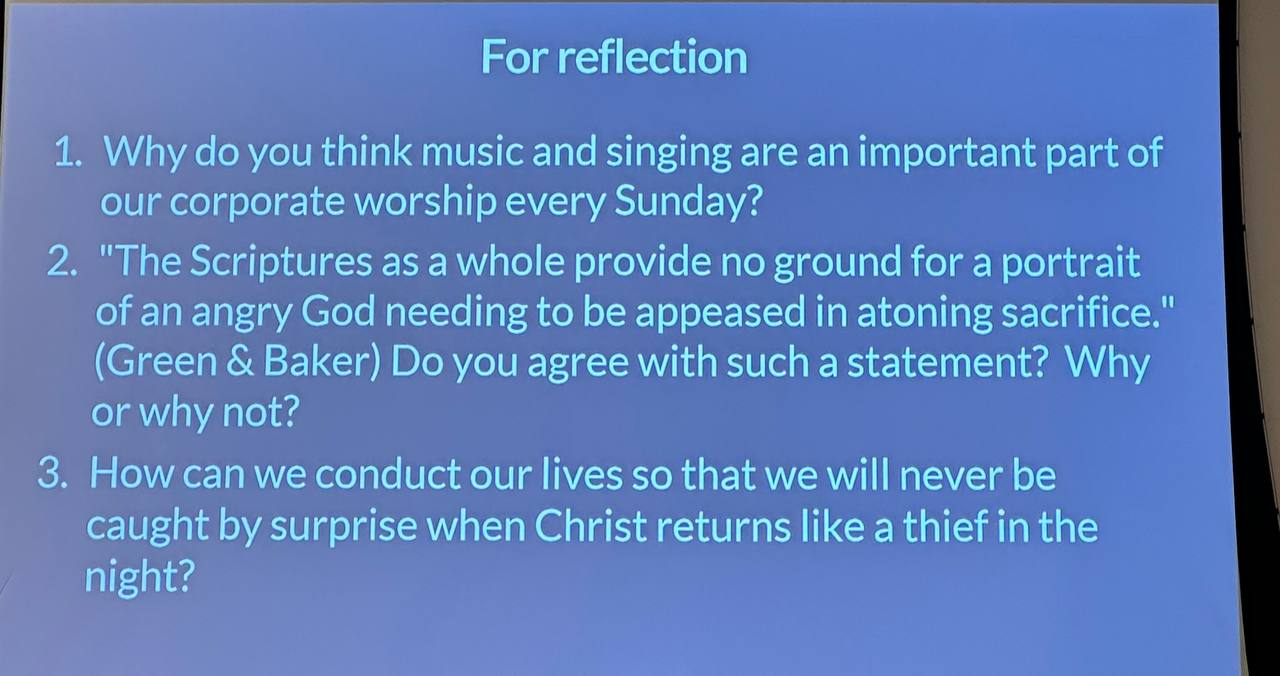
\includegraphics[width=0.8\textwidth, trim={0cm 0cm 0cm 0cm},clip]{Figures/marchSermon4Reflections.jpg}
  %   \includegraphics[width=0.8\textwidth, trim={0cm 0cm 0cm 0cm},clip]{example-image-a}
  %   \caption[]{Reflection questions for this sermon}
  %   \label{}
  % \end{figure}}
\end{itemize}